\chapter{\huge Metodo Runge-Kutta}

\textit{In analisi numerica i metodi Runge-Kutta sono una famiglia di metodi iterativi impliciti ed espliciti per la risuluzione approssimata di equazioni differenziali ordinarie (ODE). Il più comune di questi metodi è il cosidetto ``RK4'' o anche Runge-Kutta del quarto ordine.}
\\\\
Sia dato il problema di Cauchy
$$ \dot y = f(t, y), \quad y(t_0) = y_0.$$
Si assume che il tempo sia discretizzato in istanti $t_n$ equidistanziati di un intervallo $h$.\\
Il metodo RK4 per questo problema è allora dato dalle seguenti equazioni:
\begin{eqnarray*}
y_{n+1} &=& y_n + \tfrac{1}{6} \left(k_1 + 2k_2 + 2k_3 + k_4 \right)\\
t_{n+1} &=& t_n + h
\end{eqnarray*}
dove $y_{n+1}$ è l'approssimazione RK4 di $y(t_{n+1})$, e
\begin{eqnarray*}
k_1 &=& hf(t_n, y_n),\\
k_2 &=& hf(t_n + \tfrac{1}{2}h , y_n + \tfrac{1}{2} k_1),\\
k_3 &=& hf(t_n + \tfrac{1}{2}h , y_n + \tfrac{1}{2} k_2),\\
k_4 &=& hf(t_n + h , y_n + k_3).
\end{eqnarray*}
Il valore della funzione $y$ all'istante $t_{n+1}$ è uguale quindi al suo valore all'istante $t_n$ incrementato della media ponderata di quattro incrementi $k$, dove ogni incremento è il prodotto della dimensione dell'intervallo $h$ ed una stimata pendenza specificata dalla funzione $f$.
\begin{itemize}
\item $k_1$ è l'incremento basato sulla pendenza di $f$ all'estremo sinistro dell'intervallo, calcolato in $y_n$ (metodo di Eulero);
\item $k_2$ è l'incremento basato sulla pendenza nel punto medio dell'intervallo, calcolato in $y_n+\frac{1}{2}k_1$;
\item $k_3$ è ancora l'incremento basato sulla pendenza nel punto medio, calcolato però in $y_n+\frac{1}{2}k_2$;
\item $k_4$ è l'ncremento basato sulla pendenza all'estremo destro dell'intervallo, calcolato in $y_n+k_3$.
\end{itemize}
Si nota dalla formula per $y_{n+1}$ che peso maggiore viene assegnato all'incremento al centro dell'intervallo. Inoltre, se $f=f(t)$ cioè non dipende da $y$, il metodo RK4 si riduce alla regola di integrazione di Simpson.

RK4 è un metodo del quarto ordine e quindi l'errore ad ogni step è dell'ordine di $h^5$, mentre l'errore totale accumulato è dell'ordine di $h^4$.

\section{Sistemi Dinamici}
Per mezzo del metodo RK4 è possibile simulare l'evoluzione di sistemi dinamici, in particolare di quelli non lineari, le cui soluzioni non sono note analiticamente.

Esempi di sistemi dinamici che presentano comportamenti non lineari sono i sistemi di Lorenz, Rossler, Chua e di Rabinovich-Fabrikant.

\begin{figure}[H]
 \begin{subfigure}[b]{0.5\textwidth}
  \centering
  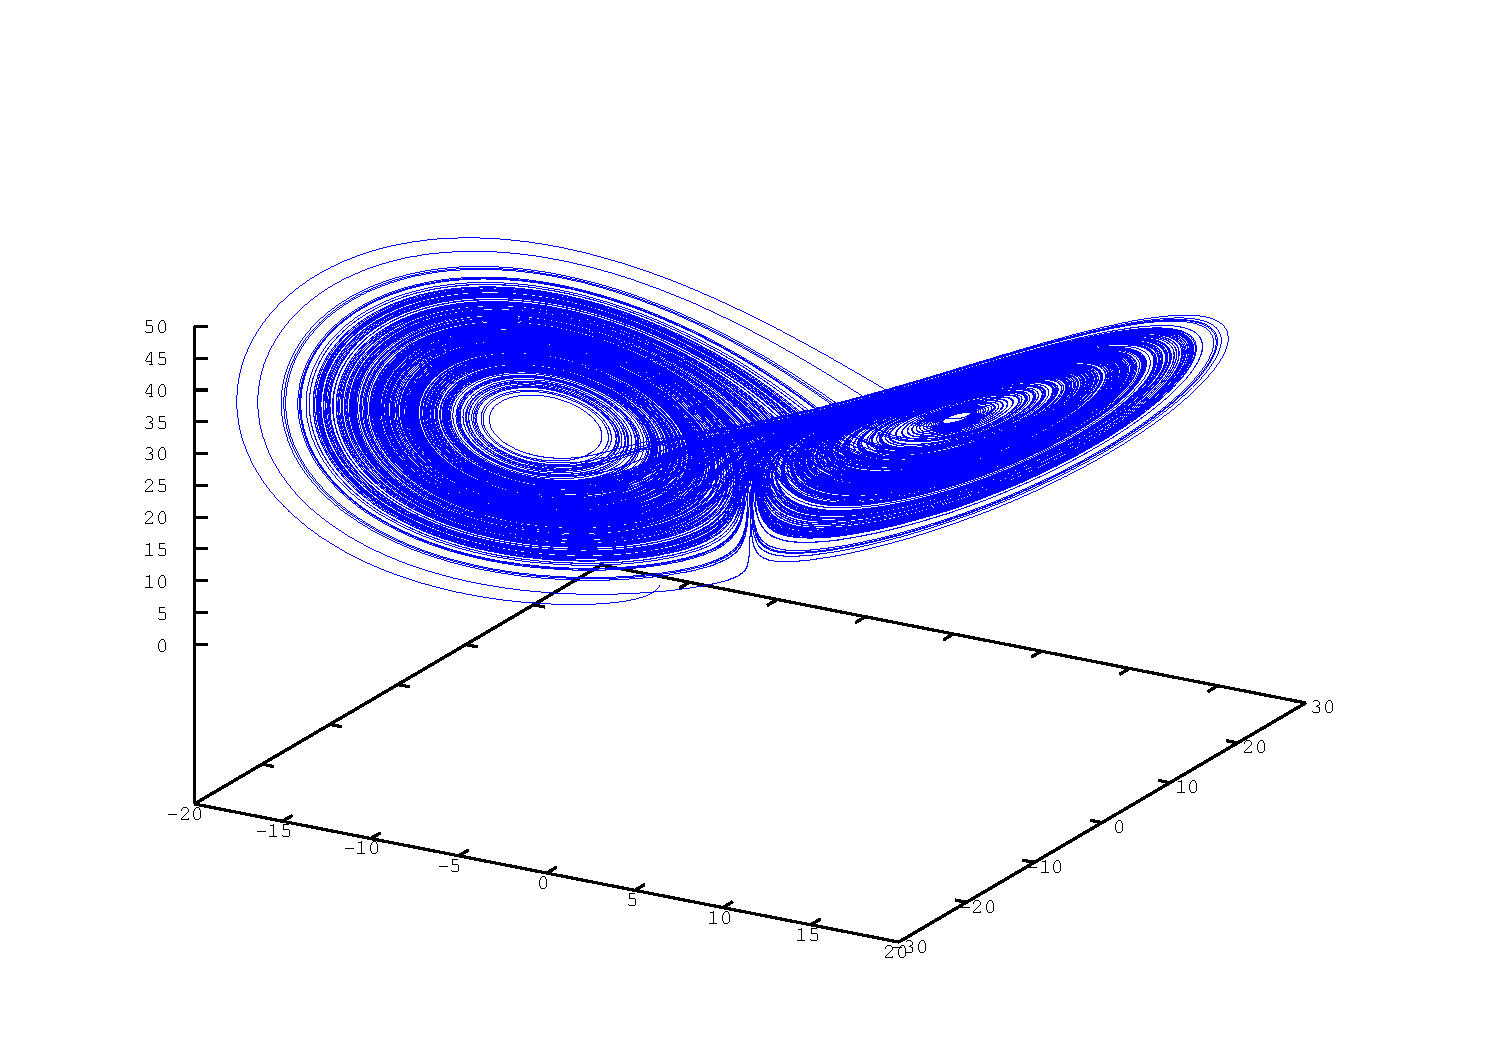
\includegraphics[width=\textwidth]{lorenz}
  \caption{Lorenz}
  \label{fig:lorenz}
 \end{subfigure}
 \begin{subfigure}[b]{0.5\textwidth}
  \centering
  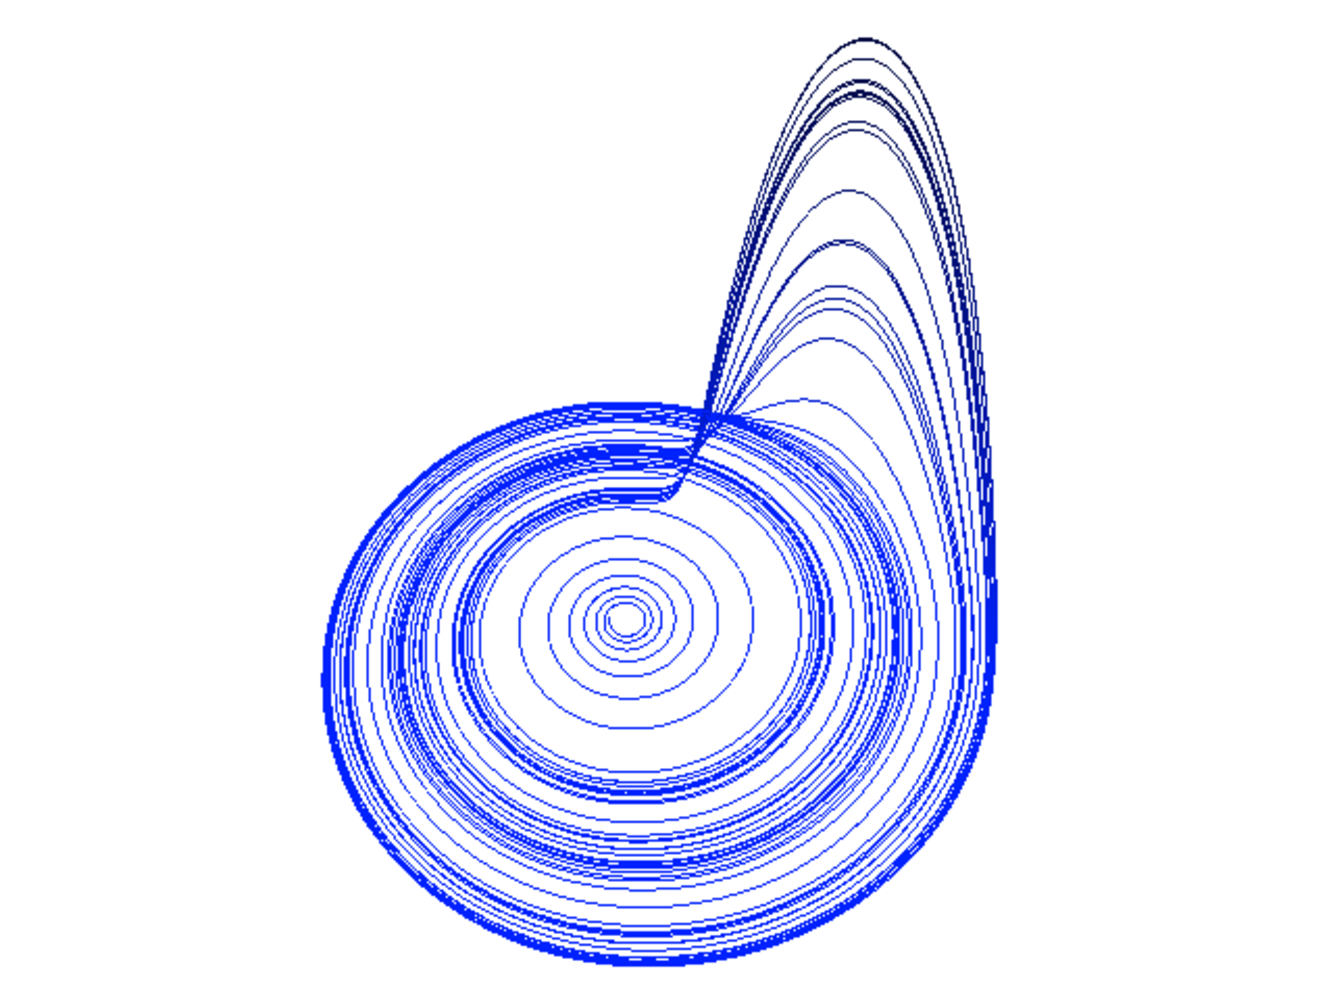
\includegraphics[width=\textwidth]{rossler}
  \caption{Rossler}
  \label{fig:rossler}
 \end{subfigure}

 \quad
 \begin{subfigure}[b]{0.5\textwidth}
  \centering
  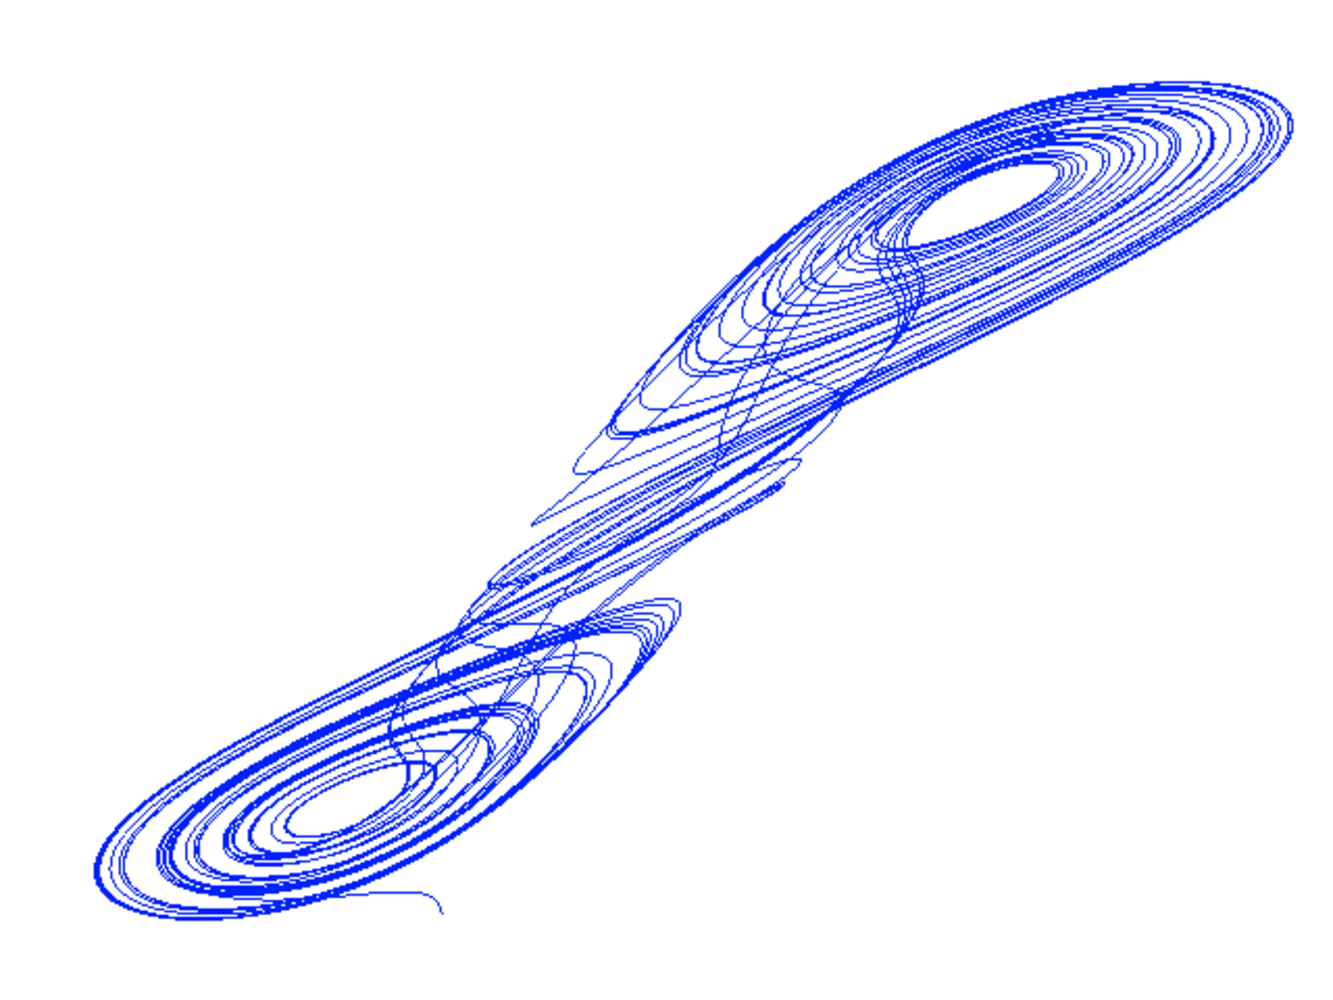
\includegraphics[width=\textwidth]{chua}
  \caption{Chua}
  \label{fig:chua}
 \end{subfigure}
 \begin{subfigure}[b]{0.5\textwidth}
  \centering
  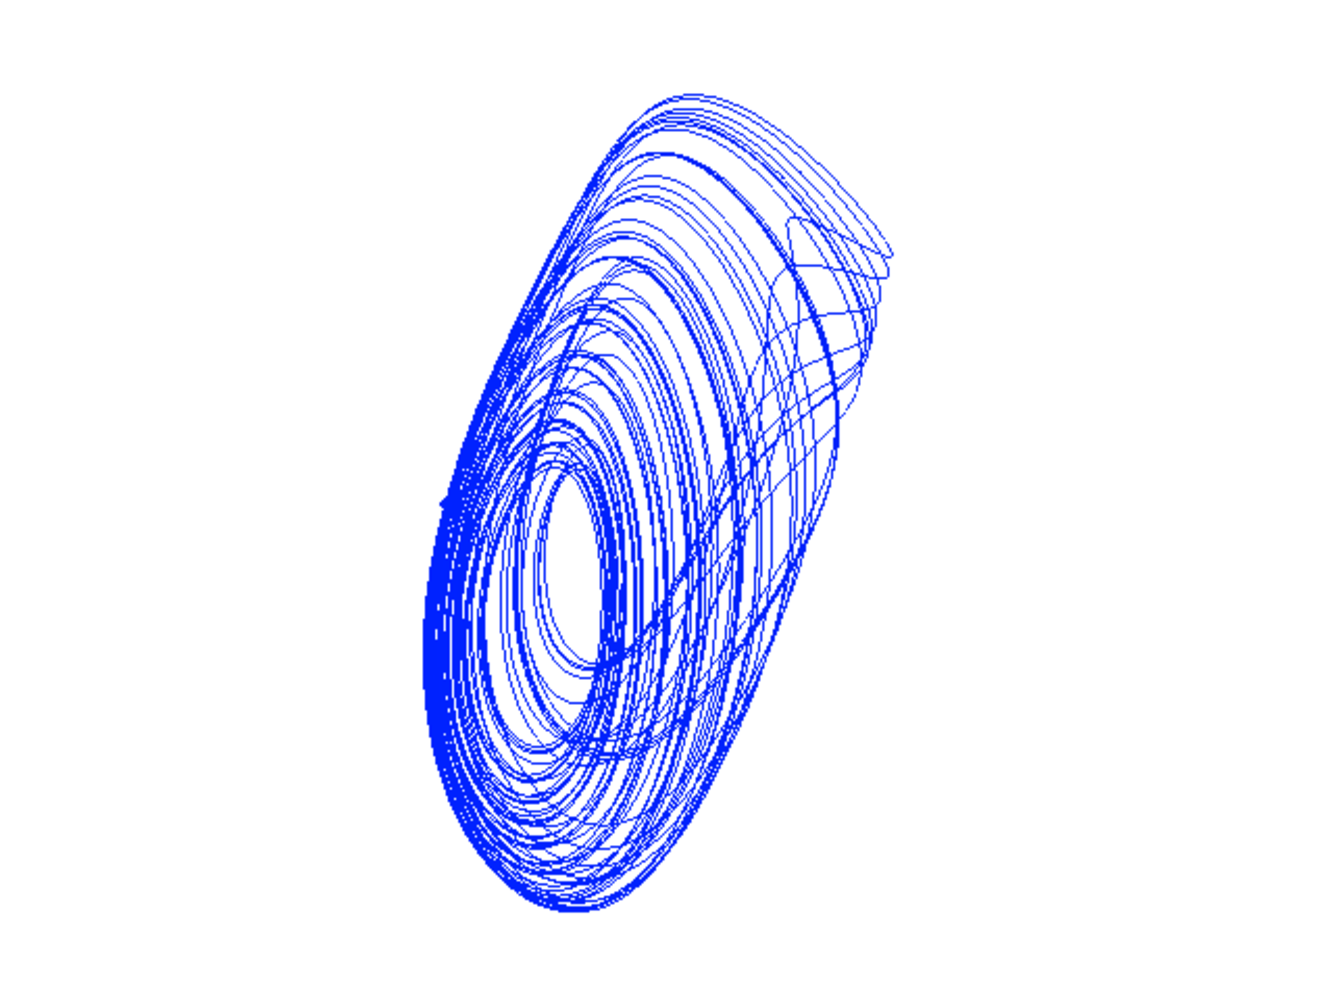
\includegraphics[width=\textwidth]{rf}
  \caption{Rabinovich-Fabrikant}
  \label{fig:rf}
 \end{subfigure}

 \caption{Soluzioni numeriche di sistemi dinamici non lineari}\label{fig:systems}
\end{figure}

